\documentclass{article}

\usepackage{listings}
\usepackage{xcolor}
\usepackage{graphicx}


\lstset{
    basicstyle=\ttfamily,
    backgroundcolor=\color{white},
    breaklines=true,
    captionpos=b,
    commentstyle=\color{green},
    keywordstyle=\color{blue},
    numberstyle=\tiny\color{gray},
    numbers=left,
    stringstyle=\color{red},
    tabsize=4,
    language=C++
}

\begin{document}

\title{Lab 3 Assignment: Report}
\author{Pradeep Mundlik}
\date{\today}
\maketitle

\begin{itemize}
    \item \textbf{Introduction:} This report provides documentation for the code related to loading data from a file and decoding RISC-V instructions. The code is organized into separate functions to achieve these tasks. Test data is stored in \texttt{data.txt} file in same directory.

    \item \textbf{Loading Data from File:} A separate function named \texttt{loadData} is implemented to load machine code values from a file. This function reads the file line by line, converts the hexadecimal strings to \texttt{uint32\_t}, and populates the vector.

    \item \textbf{Main Function:} In the main function, a vector \texttt{machineCodeList} is loaded from a text file named \texttt{data.txt}. Each line in the file contains one or more hexadecimal machine code values, which are converted into \texttt{uint32\_t} and stored in the vector.

    \item \textbf{Instruction Decoding Functions:} The code includes separate functions to decode various RISC-V instruction types, such as R, I, S, B, U, and J types. Each function extracts relevant fields from the machine code, interprets the opcode and funct3/funct7 (for R and I type), and produces the corresponding assembly instruction. If the machine code is invalid or the opcode is not recognized, appropriate error messages are displayed.

    \item \textbf{Converting \texttt{uint32\_t} to Hexadecimal Strings:} To convert a \texttt{uint32\_t} to a hexadecimal string, the code employs a stringstream named \texttt{ss}. A stringstream is an object designed for string manipulation, providing the capability to handle data as if it were a stream.
    The line \texttt{ss << hex << machineCode} effectively converts the \texttt{uint32\_t} value stored in \texttt{machineCode} to a hexadecimal string. 
    This conversion is achieved by using the \texttt{<<} operator to direct the value into the stringstream \texttt{ss}. The inclusion of the \texttt{hex} manipulator ensures that the output is formatted in hexadecimal.

    \item \textbf{For Labels in B/J type:} All disassembled instructions are stored in vector \texttt{disassembledCode}. Every time we get B/J type, we will check its next instruction according to offset value, if next instruction is already labeled then we will use that label else we will assign lable to that instruction. 
    \texttt{num\_labels} variable shows number of current labels in code and \texttt{i} variable shows number of current instruction.

    \item \textbf{Testing:} For testing, firstly I have used examples given along with problem statement. Then I have created some sample instructions and their Machine code is generated using Ripes Simulator.
    
    \begin{figure}
        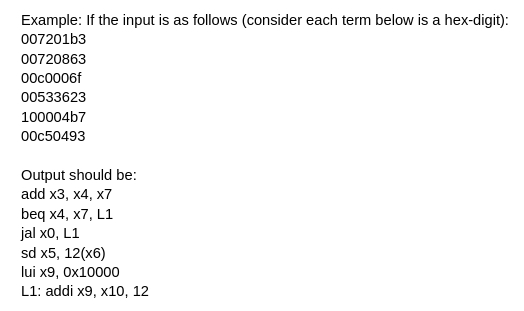
\includegraphics[width=\textwidth]{test1.png}
        \caption[short]{Sample text cases given with Assignment}
    \end{figure}
    \begin{figure}
        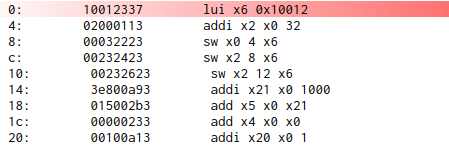
\includegraphics[width=\textwidth]{test2.png}
        \caption[short]{Sample text cases used (general)}
    \end{figure}
    \begin{figure}
        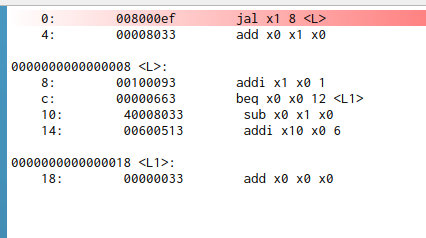
\includegraphics[width=\textwidth]{test3.png}
        \caption[short]{Sample text cases used(specific to B and J)}
    \end{figure}
\end{itemize}

\end{document}

